\clearpage
\section*{\currfilename}

\pgfdeclarelayer{background}
\pgfdeclarelayer{foreground}
\pgfsetlayers{background,main,foreground}
% Define a few styles and constants
\tikzstyle{sensor}=[draw, fill=blue!20, text width=5em, text centered, minimum height=2.5em]
\tikzstyle{ann} = [above, text width=5em]
\tikzstyle{naveqs} = [sensor, text width=6em, fill=red!20, minimum height=12em, rounded corners]
\def\blockdist{4.5}
\def\edgedist{2.5}

\begin{tikzpicture}
  \node (block3) [squareblock, label=below:{\shortstack[c]{\bf Nonlinear Equations\\ \bf of Motion}}, minimum width=6cm, inner sep=0mm] {\centering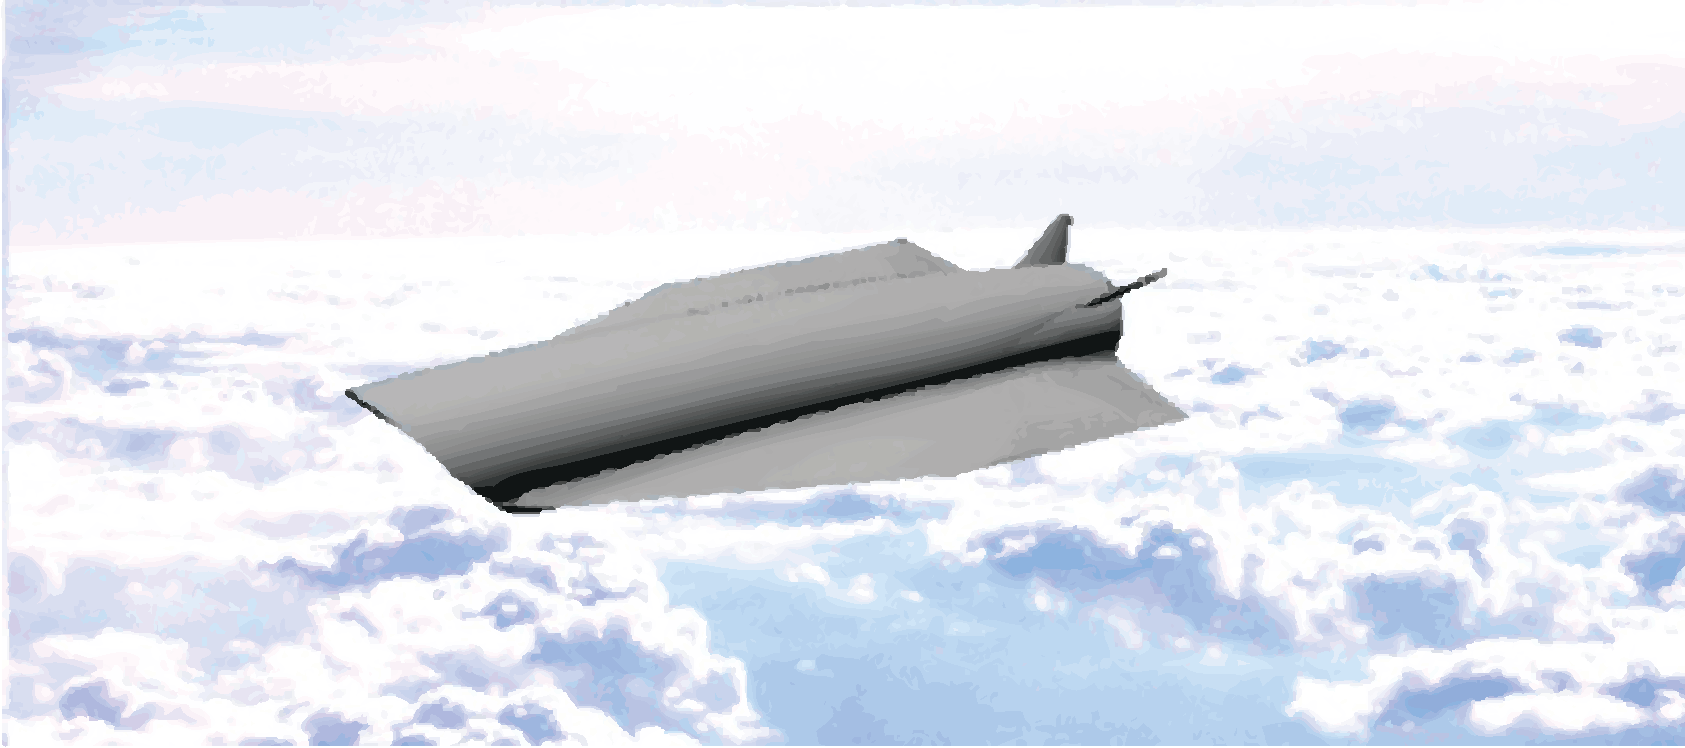
\includegraphics[width=6cm]{../fig/ghvclouds.pdf}};
  \path (naveq.145)+(-\blockdist,0) node (block1) [squareblock, minimum width=2.5cm] {Baseline};
  \path (naveq.-145)+(-\blockdist,0) node (block2) [squareblock, minimum width=2.5cm] {\shortstack{Adaptive \\ Augmentation}};
  \node[squareblock, minimum height=1cm, minimum width=2cm, right of=block3, node distance=5.0cm] (block4) {\shortstack[c]{Error \\ Generator}};
  \node[output, right of=block4,node distance=2.0cm] (output1) {};
  \path [draw, ->] (block1) -- (block3.west |- block1) ;
  \path [draw, ->] (block2) -- (block3.west |- block2);
  \draw[->](block3) -- (block4);
  \draw[->](block4) --  node[above,pos=0.8]{$e$}(output1);
\end{tikzpicture}
